%% Main presentation %%
%%%%%%%%%%%%%%%%%%%%%%%%%%%%%%%%
%%%%%%%%%%%%%%%%%%%%%%%%%%%%%%%%

%% Title slide content %%
%% Template modfied by Kirsten Wright kirsten.wright@uwaterloo.ca 2024-01-14    %%
%% Based on template by Chris Carmona: carmona@stats.ox.ac.uk ; chriscarmona.me %%

\documentclass{beamer}
% %% Packages %%
% %%%%%%%%%%%%%%%%%%%%%%%%%%%%%%%%
% %%%%%%%%%%%%%%%%%%%%%%%%%%%%%%%%

% \usepackage{tikz}
% \usepackage[UKenglish]{babel}
% \usepackage[utf8]{inputenc} % so we can input characters with accents (e.g. ő)

% \usepackage{statsbeamer}

% \usepackage{graphicx} % ease graphics management
% % \graphicspath{{images/}} % define folder with images
% % \graphicspath{{fig/}} % define folder with images
% \usefonttheme{serif} % change font to allow \textbf{}
% \usepackage{charter} % Nicer fonts

% \usepackage{amsmath,amsthm,amssymb} % for math equations

% % \usepackage{natbib} % richer citation
% \usepackage{breakcites} % avoid overfull hbox for long cites


%% Information (author, title, etc.) %%
% \setbeamerfont{title}{size*={2pt}}
\title{ Financialization of the Housing Market: A Contribution to Modern Urban Rent Theory}
% \author{Kirsten Wright} %\underline{Alyssa P. Hacker} \inst{1} \and Ben Bitdiddle \inst{2} \and Lem E. Tweakit \inst{2}}
\author{
  Author: Kirsten Wright \\
  Supervisors: Jangho Yang, Sean Geobey
}
% \institute{PhD Thesis Defensae}
\institute{PhD Thesis Defense \\[1ex] University of Waterloo}
\date{February 10, 2024}
% \title[Short Title]{% short title for footer
%     Long and Descriptive Title
%     \vspace{0.5cm}
% }
% \author{ Your Name \and Your Collaborator}
% \institute{
%         \textit{Department of Statistics}\\
%         \textit{University of Waterloo}
%         \vspace{0.5cm}
% }
% \date[Venue and Date]{% short date for footer
%     Venue, Date
% }
\begin{document}


%% Slide content %%
%%%%%%%%%%%%%%%%%%%%%%%%%%%%%%%%
%%%%%%%%%%%%%%%%%%%%%%%%%%%%%%%%

% Title slide %
% %----------------------------%
{
    \setbeamertemplate{footline}{}
    \setbeamertemplate{headline}{}
    \setbeamercolor{background canvas}{bg=white}
    \maketitle   
}

% Field spheres image %
% %----------------------------%
\begin{frame}
\begin{figure}[!ht]
\centering
\resizebox{0.85\textwidth}{!}{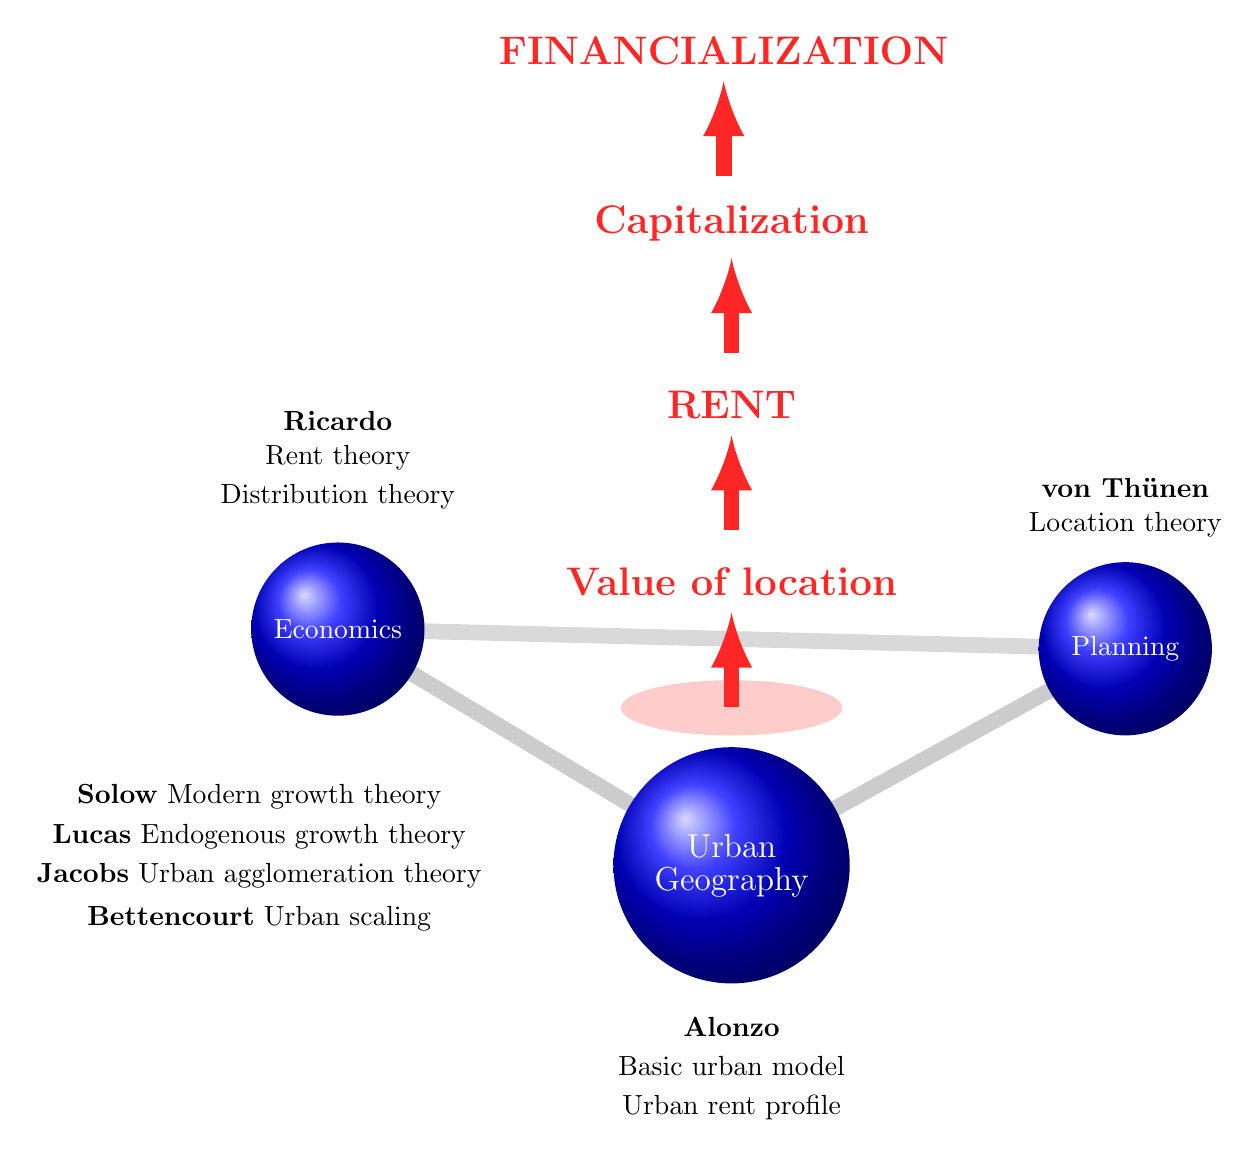
\begin{tikzpicture}{scale=.5}
% Find color for ball. Stop line short of node
\coordinate (planning) at (5,.75); % Preface
\coordinate (economics) at (-5,1); 
\coordinate (Ricardo) at (-5,1.4);
\coordinate (Solow) at (-6,1.25);
\coordinate (geography) at (0,-2); % History
\coordinate (finance) at (0,5); 

\draw [line width=2mm, black!15, ] (planning)--(economics);
\draw [line width=2mm, black!20, ] (geography)--(economics);
\draw [line width=2mm, black!20, ] (geography)--(planning);
%\draw [line width=2mm, black!25, ] (geography)--(finance);
%\draw [line width=2mm, black!20, ] (planning)--(finance);
%\draw [line width=2mm, black!20, ] (finance)--(economics);
%color=black!60!red
%\shade [ball color=blue!70] (5,5) circle (1.1cm)node[white] {\textbf{Planning}};
 
\node [circle,shading=ball,  minimum width=2.2cm, white, align=center] (ball) at (planning) {Planning};
\node [circle, shading=ball, minimum width=2.2cm, white, align=center] (ball) at (economics) {Economics};
\node [circle,shading=ball, minimum width=3cm, white, align=center] (ball) at (geography)[text width=2cm] {\large Urban \\ Geography};
%\node [circle, shading=ball, minimum width=2.4cm, white, align=center] (ball) at (finance)[text width=2cm] {Finance};
%\node at (-.3,-.1) [red] {\Large \textbf{RENT}};

\node at (planning) [above=1.8cm] {\textbf{von Th\"unen}};
\node at (planning) [above=1.3cm] {Location theory};

\node at (Ricardo) [above=2cm,]   {\textbf{Ricardo}};
\node at (Ricardo) [above=1.5cm] {Rent theory};
\node at (Ricardo) [above=1.0cm] {Distribution theory};

% \node at (Solow) [below=1.6cm, align=left] {\textbf{Solow:}};
\node at (Solow) [below=2.1cm, align=left] {\textbf{Solow} Modern growth theory};
\node at (Solow) [below=2.6cm, align=left] {\textbf{Lucas} Endogenous growth theory};
\node at (Solow) [below=3.1cm, align=left] {\textbf{Jacobs} Urban agglomeration theory};
\node at (Solow) [below=3.65cm, align=left] {\textbf{Bettencourt} Urban scaling};

\node at (geography) [below=1.8cm] {\textbf{Alonzo}};
\node at (geography) [below=2.3cm] {Basic urban model};
\node at (geography) [below=2.8cm] {Urban rent profile};
%\node [circle, shading=ball, minimum width=2.4cm, white, align=center] (ball) at (finance)[text width=2cm] {Finance};

\fill[red!20] (0,0) ellipse (40pt and 10pt);
%\node[red]at (1.2,0) {\large SPACE};
\begin{scope}[shift={(0,-.34)}]
\draw [line width=2mm, red!85, -latex ] (-.1, 7.1)--++(0,1.2)node[above=-.1] {\Large \textbf{FINANCIALIZATION}};
\draw [line width=2mm, red!85, -latex ] (0, 4.85)--++(0,1.2)node[above=-.1] {\Large \textbf{Capitalization}};
\draw [line width=2mm, red!85, -latex ] (0, 2.6)--++(0,1.2)node[above=-.1] {\Large \textbf{RENT}};
\draw [line width=2mm, red!85, -latex ] (0, .35)--++(0,1.2)node[above] {\Large \textbf{Value of location}};
%\draw [line width=2mm, red!85, -latex ] (0, -2)--++(0,-.8)node[above=-.1]  {\Large \textbf{SPACE}};
\end{scope}
\end{tikzpicture}


% % JUST THE BOTTOM 3 BALLS FOR PLANNING, ECONOMICS AND URBAN GEOGRAPHY
% \begin{figure}
% \begin{tikzpicture}{scale=.5}
% % find color cotrol for ball. Tind way to stop line short of node
% \coordinate (planning) at (-5,1);%PREFACE
% \coordinate (economics) at (5,.75);%
%  \coordinate (geography) at (-.5,-2); %history
% \coordinate (finance) at (0,5); %

% \draw [line width=2mm, black!15, ] (planning)--(economics);
% \draw [line width=2mm, black!20, ] (geography)--(economics);
% \draw [line width=2mm, black!20, ] (geography)--(planning);

% %\draw [line width=2mm, black!25, ] (geography)--(finance);
% %\draw [line width=2mm, black!20, ] (planning)--(finance);
% %\draw [line width=2mm, black!20, ] (finance)--(economics);
% \node [circle,shading=ball, minimum width=2.1   cm, white, align=center] (ball) at (planning) {Planning};
% \node [circle,shading=ball, minimum width=2.2cm, white, align=center] (ball) at (economics) {Economics};
% \node [circle,shading=ball, minimum width=3cm, white, align=center] (ball) at (geography)[text width=2cm] {\large Urban\\ Geography};
% %\node [circle, shading=ball, minimum width=2.4cm, white, align=center] (ball) at (finance)[text width=2cm] {Finance};

% \node at (-.3,-.1) [red] {\Large \textbf{Space}};
% \end{tikzpicture}
% \caption{The common concern of three fields topic }
%     \label{fig-three-fields}
% \end{figure}}
% 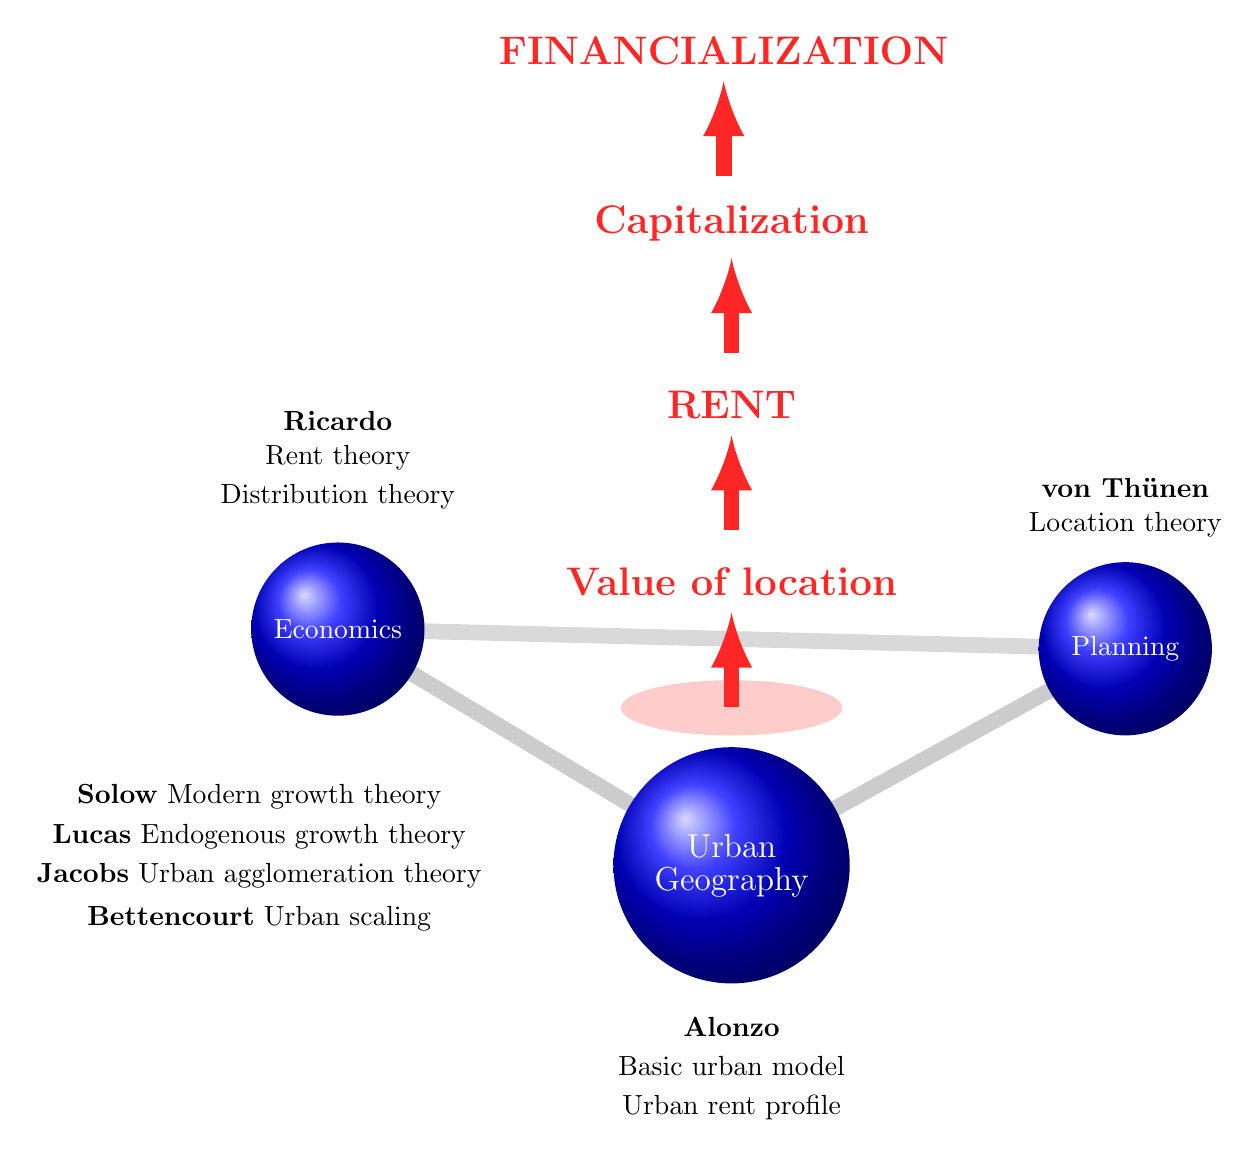
\begin{tikzpicture}{scale=.5}
% Find color for ball. Stop line short of node
\coordinate (planning) at (5,.75); % Preface
\coordinate (economics) at (-5,1); 
\coordinate (Ricardo) at (-5,1.4);
\coordinate (Solow) at (-6,1.25);
\coordinate (geography) at (0,-2); % History
\coordinate (finance) at (0,5); 

\draw [line width=2mm, black!15, ] (planning)--(economics);
\draw [line width=2mm, black!20, ] (geography)--(economics);
\draw [line width=2mm, black!20, ] (geography)--(planning);
%\draw [line width=2mm, black!25, ] (geography)--(finance);
%\draw [line width=2mm, black!20, ] (planning)--(finance);
%\draw [line width=2mm, black!20, ] (finance)--(economics);
%color=black!60!red
%\shade [ball color=blue!70] (5,5) circle (1.1cm)node[white] {\textbf{Planning}};
 
\node [circle,shading=ball,  minimum width=2.2cm, white, align=center] (ball) at (planning) {Planning};
\node [circle, shading=ball, minimum width=2.2cm, white, align=center] (ball) at (economics) {Economics};
\node [circle,shading=ball, minimum width=3cm, white, align=center] (ball) at (geography)[text width=2cm] {\large Urban \\ Geography};
%\node [circle, shading=ball, minimum width=2.4cm, white, align=center] (ball) at (finance)[text width=2cm] {Finance};
%\node at (-.3,-.1) [red] {\Large \textbf{RENT}};

\node at (planning) [above=1.8cm] {\textbf{von Th\"unen}};
\node at (planning) [above=1.3cm] {Location theory};

\node at (Ricardo) [above=2cm,]   {\textbf{Ricardo}};
\node at (Ricardo) [above=1.5cm] {Rent theory};
\node at (Ricardo) [above=1.0cm] {Distribution theory};

% \node at (Solow) [below=1.6cm, align=left] {\textbf{Solow:}};
\node at (Solow) [below=2.1cm, align=left] {\textbf{Solow} Modern growth theory};
\node at (Solow) [below=2.6cm, align=left] {\textbf{Lucas} Endogenous growth theory};
\node at (Solow) [below=3.1cm, align=left] {\textbf{Jacobs} Urban agglomeration theory};
\node at (Solow) [below=3.65cm, align=left] {\textbf{Bettencourt} Urban scaling};

\node at (geography) [below=1.8cm] {\textbf{Alonzo}};
\node at (geography) [below=2.3cm] {Basic urban model};
\node at (geography) [below=2.8cm] {Urban rent profile};
%\node [circle, shading=ball, minimum width=2.4cm, white, align=center] (ball) at (finance)[text width=2cm] {Finance};

\fill[red!20] (0,0) ellipse (40pt and 10pt);
%\node[red]at (1.2,0) {\large SPACE};
\begin{scope}[shift={(0,-.34)}]
\draw [line width=2mm, red!85, -latex ] (-.1, 7.1)--++(0,1.2)node[above=-.1] {\Large \textbf{FINANCIALIZATION}};
\draw [line width=2mm, red!85, -latex ] (0, 4.85)--++(0,1.2)node[above=-.1] {\Large \textbf{Capitalization}};
\draw [line width=2mm, red!85, -latex ] (0, 2.6)--++(0,1.2)node[above=-.1] {\Large \textbf{RENT}};
\draw [line width=2mm, red!85, -latex ] (0, .35)--++(0,1.2)node[above] {\Large \textbf{Value of location}};
%\draw [line width=2mm, red!85, -latex ] (0, -2)--++(0,-.8)node[above=-.1]  {\Large \textbf{SPACE}};
\end{scope}
\end{tikzpicture}


% % JUST THE BOTTOM 3 BALLS FOR PLANNING, ECONOMICS AND URBAN GEOGRAPHY
% \begin{figure}
% \begin{tikzpicture}{scale=.5}
% % find color cotrol for ball. Tind way to stop line short of node
% \coordinate (planning) at (-5,1);%PREFACE
% \coordinate (economics) at (5,.75);%
%  \coordinate (geography) at (-.5,-2); %history
% \coordinate (finance) at (0,5); %

% \draw [line width=2mm, black!15, ] (planning)--(economics);
% \draw [line width=2mm, black!20, ] (geography)--(economics);
% \draw [line width=2mm, black!20, ] (geography)--(planning);

% %\draw [line width=2mm, black!25, ] (geography)--(finance);
% %\draw [line width=2mm, black!20, ] (planning)--(finance);
% %\draw [line width=2mm, black!20, ] (finance)--(economics);
% \node [circle,shading=ball, minimum width=2.1   cm, white, align=center] (ball) at (planning) {Planning};
% \node [circle,shading=ball, minimum width=2.2cm, white, align=center] (ball) at (economics) {Economics};
% \node [circle,shading=ball, minimum width=3cm, white, align=center] (ball) at (geography)[text width=2cm] {\large Urban\\ Geography};
% %\node [circle, shading=ball, minimum width=2.4cm, white, align=center] (ball) at (finance)[text width=2cm] {Finance};

% \node at (-.3,-.1) [red] {\Large \textbf{Space}};
% \end{tikzpicture}
% \caption{The common concern of three fields topic }
%     \label{fig-three-fields}
% \end{figure}
% \includegraphics[width=0.6\textwidth]{fig/fields}
% \caption[Linking space and urban rents to the effects of financialization.]{Space and urban rents play a foundational role in urban economics, geography, and planning. We extend the analysis of urban rents to model the effects of financialization.}
\label{fig-fields}
\end{figure}
\end{frame}

% %----------------------------%
\begin{frame}%{The housing market component}
\begin{center}
    
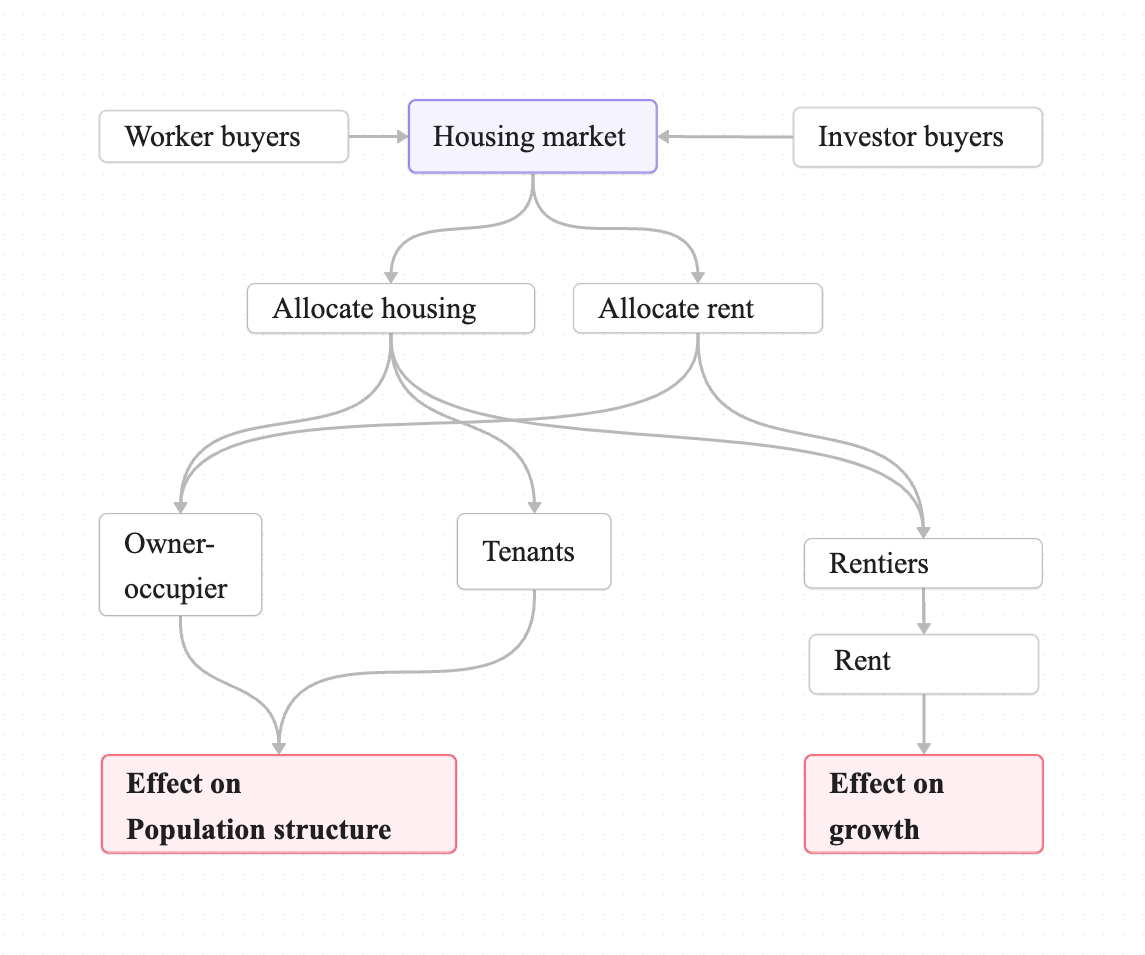
\includegraphics[scale=.55]{fig/flow-impacts.png}
\end{center}

% \caption[The housing market component of the model.]{The housing market component. Financialization affects both the allocation of housing and its allocation of rents.}
\end{frame}

% %----------------------------%
\begin{frame}{The financialization component}
% \begin{figure}[!ht]
\centering
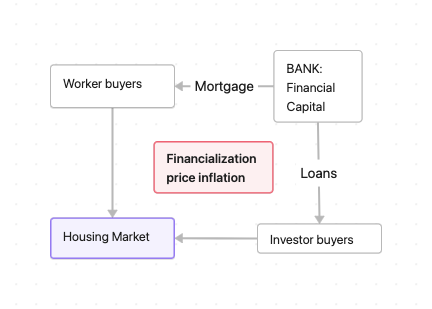
\includegraphics[scale=.55]{fig/flow-financialization.png}
% \caption[The financialization component of the model.]{The financialization component. There is a feedback loop in which new investors drive up demand and thus drive up prices.}
% \label{fig-financial-cycle}
% \end{figure}
\end{frame}

% %----------------------------%
\begin{frame}{The production system}
% \begin{figure}[!ht]
\centering
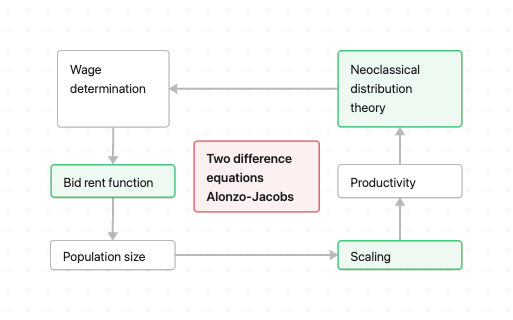
\includegraphics[scale=.55]{fig/flow-alonso-jacobs-cycle.png}
% \caption[Production system.]{The production system component, incorporating the urban scaling of wealth in the urban spatial model. We name this coupling of two difference equations the Alonso-Jacobs cycle.}
% \label{fig-alonso-jacobs-cycle}
% \end{figure}
\end{frame}

% %----------------------------%
\begin{frame}{Frame Title}
\end{frame}

% %----------------------------%
% %----------------------------%
% %----------------------------%
% %----------------------------%
% %----------------------------%
% %----------------------------%
% %----------------------------%
% %----------------------------%
% %----------------------------%
% %----------------------------%
% %----------------------------%
% %----------------------------%
% %----------------------------%
% %----------------------------%
% %----------------------------%
% %----------------------------%
% %----------------------------%
% %----------------------------%
% %----------------------------%
% %----------------------------%
% %----------------------------%
% %----------------------------%
% %----------------------------%
% %----------------------------%
% %----------------------------%
% %----------------------------%
% %----------------------------%
% %----------------------------%
% %----------------------------%
% %----------------------------%
% %----------------------------%
% %----------------------------%
% %----------------------------%
% %----------------------------%
% %----------------------------%
% %----------------------------%
% %----------------------------%
% %----------------------------%
% %----------------------------%
% %----------------------------%
% %----------------------------%
% %----------------------------%
% %----------------------------%
% %----------------------------%
% %----------------------------%


%% Example content %%
%%%%%%%%%%%%%%%%%%%%%%%%%%%%%%%%
%%%%%%%%%%%%%%%%%%%%%%%%%%%%%%%%

% %----------------------------%
% % Contents slide
% \begin{frame}
% \frametitle{Outline}
% \tableofcontents
% \end{frame}
% %----------------------------%

% %now include the slides
% \setbeamercovered{transparent}
% %----------------------------%
% \section{Section 1}
% \subsection{Subsection a}

% \begin{frame}
%     \frametitle{First slide Title}
%     \small
%     Add your contents and citations %\citep{Tantau2016beamerguide}
% \end{frame}
% \section{Section 2}
% \begin{frame}
%     \frametitle{Another Slide}
%     \small
%     Maybe some figures like Fig.~\ref{fig:my_label}
%     \begin{figure}
%         \centering
%         \includegraphics[width=3cm]{example-image-a}
%         \caption{Example image}
%         \label{fig:my_label}
%     \end{figure}
% \end{frame}
% %----------------------------%

% %----------------------------%
% % Conclusions
% \begin{frame}
%     \frametitle{}
%     \centering
    
%     \Large\color{titlecolor}
%     Thank you!

%     \vspace{0.5cm}
%     kirsten.wright@uwaterloo.ca

% \end{frame}
% %----------------------------%

% % References slide
% \begin{frame}
% \frametitle{References}
% \small
% % \bibliographystyle{apalike} %use the apalike bibliography style
% \bibliography{thesis-bib} % bibliography file
% \end{frame}

\end{document}
%%%%%%%%%%%%%%%%%%%%%%%%%%%%%%%%
%%%%%%%%%%%%%%%%%%%%%%%%%%%%%%%%